% Number the handout's main topics as 1, 2, 3, ... within this lab.
\renewcommand{\thesubsection}{\arabic{subsection}}
\renewcommand{\thesubsubsection}{\thesubsection.\arabic{subsubsection}}
\section{A cooperative scheduler}

\subsection{Introduction}
\subsubsection{Super Loop Architecture}
\begin{lstlisting}[basicstyle=\small, caption=Super loop program,label = {program_super_loop}]
}
void main(void){
    // Prepare for Task X
    X_Init();
    while(1) {// 'for ever' (Super Loop)
        X(); // Perform the task
    } 
}
\end{lstlisting}
The main advantages of the Super Loop architecture illustrated above are:
\begin{itemize}
    \item (1) that it is simple, and therefore easy to understand, and 
    \item (2) that it consumes virtually no system memory or CPU resources.
\end{itemize}

However, we get ‘nothing for nothing’: Super Loops consume little memory or
processor resources because they provide few facilities to the developer. A particular
limitation with this architecture is that it is very difficult to execute Task X at precise
intervals of time: as we will see, this is a very significant drawback.

For example, consider a collection of requirements assembled from a range of different embedded projects (in no particular order):
\begin{itemize}
    \item The current speed of the vehicle must be measured at 0.5 second intervals.
    \item The display must be refreshed 40 times every second. 
    \item The calculated new throttle setting must be applied every 0.5 seconds.
    \item A time-frequency transform must be performed 20 times every second.
    \item If the alarm sounds, it must be switched off (for legal reasons) after 20 minutes.
    \item If the front door is opened, the alarm must sound in 30 seconds if the correct
password is not entered in this time.    
\item The engine vibration data must be sampled 1,000 times per second.
    \item The frequency-domain data must be classified 20 times every second.
    \item The keypad must be scanned every 200 ms.
    \item The master (control) node must communicate with all other nodes (sensor nodes
and sounder nodes) once per second.
    \item The new throttle setting must be calculated every 0.5 seconds. 
    \item The sensors must be sampled once per second.
\end{itemize}

We can summarize this list by saying that many embedded systems must carry
out tasks at particular instants of time. More specifically, we have two kinds of activity to perform:
\begin{itemize}
    \item Periodic tasks, to be performed (say) once every 100 ms
    \item One-shot tasks, to be performed once after a delay of (say) 50 ms  
\end{itemize}

This is very difficult to achieve with the primitive architecture shown in Program above. Suppose, for example, that we need to start Task X every 200 ms, and that the
task takes 10 ms to complete. Program below illustrates one way in which we might
adapt the code in order to try to achieve this.

\begin{lstlisting}[basicstyle=\small, caption= Trying to use the Super Loop architecture to execute tasks at regular intervals, label = {program_super_loop}]
}
void main(void){
    // Prepare for Task X
    X_Init();
    while(1) {          // 'for ever' (Super Loop)
        X();            // Perform the task (10 ms duration)
        Delay_190ms();  // Delay for 190 ms
    } 
}
\end{lstlisting}

The approach is not generally adequate, because it will only work if the following conditions are satisfied:
\begin{itemize}
    \item We know the precise duration of Task X
    \item This duration never varies
\end{itemize}

In practical applications, determining the precise task duration is rarely straightforward. Suppose we have a very simple task that does not interact with the outside
world but, instead, performs some internal calculations. Even under these rather
restricted circumstances, changes to compiler optimization settings – even changes to
an apparently unrelated part of the program – can alter the speed at which the task
executes. This can make fine-tuning the timing very tedious and error prone.

The second condition is even more problematic. Often in an embedded system the
task will be required to interact with the outside world in a complex way. In these circumstances the task duration will vary according to outside activities in a manner
over which the programmer has very little control.


\subsubsection{Timer-based interrupts and interrupt service routines}
A better solution to the problems outlined is to use timer-based interrupts as a means
of invoking functions at particular times.

An interrupt is a hardware mechanism used to notify a processor that an ‘event’ has taken place: such events may be internal events or external events.


When an interrupt is generated, the processor ‘jumps’ to an address at the bottom
of the CODE memory area. These locations must contain suitable code with which
the microcontroller can respond to the interrupt or, more commonly, the locations
will include another ‘jump’ instruction, giving the address of suitable ‘interrupt service routine’ located elsewhere in (CODE) memory.

Please see lab 3 for the more information of this approach. 

\subsection{What is a scheduler?}
There are two ways of viewing a scheduler:
\begin{itemize}
    \item  At one level, a scheduler can be viewed as a simple operating system that allows
tasks to be called periodically or (less commonly) on a one-shot basis.  
    \item  At a lower level, a scheduler can be viewed as a single timer interrupt service routine that is shared between many different tasks. As a result, only one timer needs to be  initialized, and any changes to the timing generally requires only one function to be altered. Furthermore, we can generally use the same scheduler whether we need to execute one, ten or 100 different tasks. 

\end{itemize}
\begin{lstlisting}[caption=Example of how a scheduler uses]
void main(void) {
    // Set up the scheduler
    SCH_Init();
    // Add the tasks (1ms tick interval)
    // Function_A will run every 2 ms
    SCH_Add_Task(Function_A, 0, 2);
    // Function_B will run every 10 ms
    SCH_Add_Task(Function_B, 1, 10);
    // Function_C will run every 15 ms
    SCH_Add_Task(Function_C, 3, 15);
    while(1) {
        SCH_Dispatch_Tasks();
    } 
}
\end{lstlisting}

\subsubsection{The co-operative scheduler}

● A co-operative scheduler provides a single-tasking system architecture

\textbf{Operation}:
\begin{itemize}
    \item Tasks are scheduled to run at specific times (either on a periodic or one-shot basis)
\item When a task is scheduled to run it is added to the waiting list
\item When the CPU is free, the next waiting task (if any) is executed
\item The task runs to completion, then returns control to the scheduler
\end{itemize}


\textbf{Implementation}:
\begin{itemize}
    \item The scheduler is simple and can be implemented in a small amount of code
    \item The scheduler must allocate memory for only a single task at a time
    \item The scheduler will generally be written entirely in a high-level language (such as ‘C’)
   \item The scheduler is not a separate application; it becomes part of the developer’s code
\end{itemize}


\textbf{Performance}:
\begin{itemize}
    \item Obtaining rapid responses to external events requires care at the design stage
Reliability and safety:

\end{itemize}

\textbf{Co-operate scheduling is simple, predictable, reliable and safe}

A co-operative scheduler provides a simple, highly predictable environment. The
scheduler is written entirely in ‘C’ and becomes part of the application: this tends to
make the operation of the whole system more transparent and eases development,
maintenance and porting to different environments. Memory overheads are 17
bytes per task and CPU requirements (which vary with tick interval) are low.

\subsubsection{Function pointers}
One area of the language with which many `C' programmers are unfamiliar is the
function pointer. While comparatively rarely used in desktop programs, this language
feature is crucial in the creation of schedulers: we therefore provide a brief introductory example here.

The key point to note is that – just as we can, for example, determine the starting
address of an array of data in memory – we can also find the address in memory at
which the executable code for a particular function begins. This address can be used
as a ‘pointer’ to the function; most importantly, it can be used to call the function.
Used with care, function pointers can make it easier to design and implement complex programs. For example, suppose we are developing a large, safety-critical,
application, controlling an industrial plant. If we detect a critical situation, we may
wish to shut down the system as rapidly as possible. However, the appropriate way to
shut down the system will vary, depending on the system state. What we can do is
create a number of different recovery functions and a function pointer. Every time
the system state changes, we can alter the function pointer so that it is always pointing to the most appropriate recovery function. In this way, we know that – if there is
ever an emergency situation – we can rapidly call the most appropriate function, by
means of the function pointer.

\begin{lstlisting}[basicstyle=\small, caption=Example of how to use function pointers]
// ------ Private function prototypes -----------------------------
void Square_Number(int, int*);

int main(void)
{
    int a = 2, b = 3; 
    /* Declares pFn to be a pointer to fn with 
    int and int pointer parameters (returning void) */
    void (* pFn)(int, int*);
    
    int Result_a, Result_b;
    pFn = Square_Number; // pFn holds address of Square_Number
    printf("Function code starts at address: %u\n", (tWord) pFn);
    printf("Data item a starts at address: %u\n\n", (tWord) &a);
    // Call `Square_Number' in the conventional way
    Square_Number(a, &Result_a);
    // Call `Square_Number' using function pointer
    (*pFn)(b,&Result_b);
    printf("%d squared is %d (using normal fn call)\n", a, Result_a); 
    printf("%d squared is %d (using fn pointer)\n", b, Result_b); 
    while(1);
    return 0;
}

void Square_Number(int a, int* b)
{// Demo - calculate square of a
    *b = a * a;
}
\end{lstlisting}

\subsubsection{Solution}
A scheduler has the following key components:
\begin{itemize}
    \item  The scheduler data structure.
    \item  An initialization function.
    \item  A single interrupt service routine (ISR), used to update the scheduler at regular time
    intervals.
    \item  A function for adding tasks to the scheduler.
    \item  A dispatcher function that causes tasks to be executed when they are due to run.
    \item  A function for removing tasks from the scheduler (not required in all applications).
\end{itemize}

We consider each of the required components in this section

\subsubsection{Overview}
Before discussing the scheduler components, we consider how the scheduler will
typically appear to the user. To do this we will use a simple example: a scheduler used
to flash a single LED on and off repeatedly: on for one second off for one second etc.
\begin{lstlisting}[basicstyle=\small, caption=Example of how to use a scheduler]
int main(void){
    //Init all the requirments for the system to run
	System_Initialization();
	//Init a schedule
	SCH_Init();
	//Add a task to repeatly call in every 1 second.
	SCH_Add_Task(Led_Display, 0, 1000);
	while (1){
		SCH_Dispatch_Tasks();
	}
	return 0;
}
\end{lstlisting}
\begin{itemize}
    \item We assume that the LED will be switched on and off by means of a ‘task’
Led\_Display(). Thus, if the LED is initially off and we call
Led\_Display() twice, we assume that the LED will be switched on and
then switched off again. 

To obtain the required flash rate, we therefore require that the scheduler calls
Led\_Display() every second ad infinitum.

    \item We prepare the scheduler using the function SCH\_Init().
    \item After preparing the scheduler, we add the function Led\_Display() to the
scheduler task list using the SCH\_Add\_Task() function. At the same time we specify that the LED will be turned on and off at the required rate as follows:

\textbf{SCH\_Add\_Task(Led\_Display, 0, 1000);}

We will shortly consider all the parameters of SCH\_Add\_Task(), and examine its
internal structure.

\item The timing of the Led\_Display() function will be controlled by the function
SCH\_Update(), an interrupt service routine triggered by the overflow of Timer 2:
\begin{lstlisting}[basicstyle=\small, caption=Example of how to call SCH\_Update function]
void HAL_TIM_PeriodElapsedCallback(TIM_HandleTypeDef *htim){
	SCH\_Update();
}
\end{lstlisting}

\item The ‘Update’ function does not execute the task: it calculates when a task is due to run and sets a flag. The job of executing LED\_Display() falls to the dispatcher
function (SCH\_Dispatch\_Tasks()), which runs in the main (‘super’) loop:
\begin{lstlisting}
while(1){
    SCH_Dispatch_Tasks();
}
\end{lstlisting}

\end{itemize}

Before considering these components in detail, we should acknowledge that this is,
undoubtedly, a complicated way of flashing an LED: if our intention were to develop
an LED flasher application that requires minimal memory and minimal code size,
this would not be a good solution. However, the key point is that we will be able to
use the same scheduler architecture in all our subsequent examples, including a
number of substantial and complex applications and the effort required to understand the operation of this environment will be rapidly repaid.

It should also be emphasized that the scheduler is a ‘low-cost’ option: it consumes
a small percentage of the CPU resources (we will consider precise percentages shortly).
In addition, the scheduler itself requires no more than 17 bytes of memory for each
task. Since a typical application will require no more than four to six tasks, the task –
memory budget (around 60 bytes) is not excessive, even on an 8-bit microcontroller.

\subsubsection{The scheduler data structure and task array}
At the heart of the scheduler is the scheduler data structure: this is a user-defined data
type which collects together the information required about each task.

\begin{lstlisting}[basicstyle=\small, caption=A struct of a task]

typedef struct {
    // Pointer to the task (must be a 'void (void)' function)
	void ( * pTask)(void);
	// Delay (ticks) until the function will (next) be run
	uint32_t Delay;
	// Interval (ticks) between subsequent runs.
	uint32_t Period;
	// Incremented (by scheduler) when task is due to execute
	uint8_t RunMe;
	//This is a hint to solve the question below.
	uint32_t TaskID;
} sTask;

// MUST BE ADJUSTED FOR EACH NEW PROJECT
#define SCH_MAX_TASKS 			40
#define	NO_TASK_ID				0
sTask SCH_tasks_G[SCH_MAX_TASKS];
\end{lstlisting}

\textbf{The size of the task array}

You must ensure that the task array is sufficiently large to store the tasks required in
your application, by adjusting the value of SCH\_MAX\_TASKS.
For example, if you schedule three tasks as follows:
\begin{itemize}
    \item SCH\_Add\_Task(Function\_A, 0, 2);
    \item SCH\_Add\_Task(Function\_B, 1, 10);
    \item SCH\_Add\_Task(Function\_C, 3, 15);
\end{itemize}


then SCH\_MAX\_TASKS must have a value of three (or more) for correct operation of
the scheduler.

Note also that, if this condition is not satisfied, the scheduler should generate an
error code.
\subsubsection{The initialization function}
Like most of the tasks we wish to schedule, the scheduler itself requires an initialization function. While this performs various important operations – such as preparing
the scheduler array (discussed earlier) and the error code variable (discussed later) –
the main purpose of this function is to set up a timer that will be used to generate the
regular ‘ticks’ that will drive the scheduler.

\begin{lstlisting}[basicstyle=\small, caption=Example of how]
void SCH_Init(void) {
    unsigned char i;
    for (i = 0; i < SCH_MAX_TASKS; i++) {
        SCH_Delete_Task(i);
    }
    // Reset the global error variable
    // - SCH_Delete_Task() will generate an error code, 
    // (because the task array is empty)
    Error_code_G = 0;
    Timer_init();
    Watchdog_init();
}
\end{lstlisting}
\subsubsection{The ‘Update’ function}
The ‘Update’ function is involved in the ISR. It is invoked when the timer is overflow.

When it determines that a task is due to run, the update function increments the
RunMe field for this task: the task will then be executed by the dispatcher, as we discuss later.
\begin{lstlisting}[basicstyle=\small, caption=Example of how to write an SCH\_Update function]
void SCH_Update(void){
    unsigned char Index;
    // NOTE: calculations are in *TICKS* (not milliseconds)
    for (Index = 0; Index < SCH_MAX_TASKS; Index++) {
        // Check if there is a task at this location
        if (SCH_tasks_G[Index].pTask){
            if (SCH_tasks_G[Index].Delay == 0) {
                // The task is due to run
                // Inc. the 'RunMe' flag
                SCH_tasks_G[Index].RunMe += 1; 
                if (SCH_tasks_G[Index].Period) {
                    // Schedule periodic tasks to run again
                    SCH_tasks_G[Index].Delay = SCH_tasks_G[Index].Period;
                } 
            } else {
                // Not yet ready to run: just decrement the delay 
                SCH_tasks_G[Index].Delay -= 1;
            }
        } 
    }
}

void HAL_TIM_PeriodElapsedCallback(TIM_HandleTypeDef *htim) {
	SCH_Update();
}

\end{lstlisting}

\subsubsection{The ‘Add Task’ function}
As the name suggests, the ‘Add Task’ function is used to add tasks to the task array, to
ensure that they are called at the required time(s).
Here is the example of add task function: 
\textbf{unsigned   char   SCH\_Add\_Task ( Task\_Name  , Initial\_Delay, Period )}

The parameters for the ‘Add Task’ function are described as follows:
\begin{itemize}
    \item \textbf{Task\_Name}: the name of the function (task) that you wish to schedule 
    \item \textbf{Initial\_Delay}: the delay (in ticks) before task is first executed. If set to 0,
the task is executed immediately.
    \item \textbf{Period}: the interval (in ticks) between repeated executions of the task. If set to 0, the task is executed only once
    
\end{itemize}

Here are some examples.

This set of parameters causes the function Do\_X() to be executed once after 1,000
scheduler ticks:

\textbf{SCH\_Add\_Task(Do\_X,1000,0);}

This does the same, but saves the task ID (the position in the task array) so that the
task may be subsequently deleted, if necessary (see SCH\_Delete\_Task() for further
information about the removal of tasks from the task array):

\textbf{Task\_ID = SCH\_Add\_Task(Do\_X,1000,0);}

This causes the function Do\_X() to be executed regularly every 1,000 scheduler ticks;
the task will first be executed as soon as the scheduling is started:


\textbf{SCH\_Add\_Task(Do\_X,0,1000);}

This causes the function Do\_X() to be executed regularly every 1,000 scheduler
ticks; task will be first executed at T = 300 ticks, then 1,300, 2,300 etc:

\textbf{SCH\_Add\_Task(Do\_X,300,1000);}

\begin{lstlisting}[basicstyle=\small, caption=An implementation of the scheduler ‘add task’ function]
/*------------------------------------------------------------------*-
SCH_Add_Task() Causes a task (function) to be executed at regular intervals 
or after a user-defined delay
-*------------------------------------------------------------------*/
unsigned char SCH_Add_Task(void (* pFunction)(), unsigned int DELAY, unsigned int PERIOD) 
{
    unsigned char Index = 0;
    // First find a gap in the array (if there is one)
    while ((SCH_tasks_G[Index].pTask != 0) && (Index < SCH_MAX_TASKS))
    {
       Index++;
    } 
    // Have we reached the end of the list? 
    if (Index == SCH_MAX_TASKS)
    {
        // Task list is full
        // Set the global error variable
        Error_code_G = ERROR_SCH_TOO_MANY_TASKS;
        // Also return an error code
        return SCH_MAX_TASKS; 
    }
    // If we're here, there is a space in the task array
    SCH_tasks_G[Index].pTask = pFunction;
    SCH_tasks_G[Index].Delay = DELAY;
    SCH_tasks_G[Index].Period = PERIOD;
    SCH_tasks_G[Index].RunMe = 0;
    // return position of task (to allow later deletion)
    return Index; 
}
\end{lstlisting}


\subsubsection{The ‘Dispatcher’}
As we have seen, the ‘Update’ function does not execute any tasks: the tasks that are
due to run are invoked through the ‘Dispatcher’ function.

\begin{lstlisting}[basicstyle=\small, caption=An implementation of the scheduler ‘dispatch task’ function]
void SCH_Dispatch_Tasks(void) 
{
    unsigned char Index;
    // Dispatches (runs) the next task (if one is ready)
    for (Index = 0; Index < SCH_MAX_TASKS; Index++){
        if (SCH_tasks_G[Index].RunMe > 0) {
            (*SCH_tasks_G[Index].pTask)(); // Run the task
            SCH_tasks_G[Index].RunMe -= 1; // Reset / reduce RunMe flag
            // Periodic tasks will automatically run again
            // - if this is a 'one shot' task, remove it from the array
            if (SCH_tasks_G[Index].Period == 0)
            {
                SCH_Delete_Task(Index);
            }
        } 
    }
    // Report system status
    SCH_Report_Status(); 
    // The scheduler enters idle mode at this point 
    SCH_Go_To_Sleep(); 
}
\end{lstlisting}

The dispatcher is the only component in the Super Loop:
\begin{lstlisting} [basicstyle=\small, caption= The dispatcher in the super loop]
void main(void)
{
    ...
    while(1)
    {
        SCH_Dispatch_Tasks();
    }
\end{lstlisting}

\textbf{Do we need a Dispatch function?}

At first inspection, the use of both the ‘Update’ and ‘Dispatch’ functions may seem a
rather complicated way of running the tasks. Specifically, it may appear that the
Dispatch function in unnecessary and that the Update function could invoke the
tasks directly. However, the split between the Update and Dispatch operations is necessary, to maximize the reliability of the scheduler in the presence of long tasks.

Suppose we have a scheduler with a tick interval of 1 ms and, for whatever reason,
a scheduled task sometimes has a duration of 3 ms.

If the Update function runs the functions directly then – all the time the long task
is being executed – the tick interrupts are effectively disabled. Specifically, two ‘ticks’
will be missed. This will mean that all system timing is seriously affected and may
mean that two (or more) tasks are not scheduled to execute at all.

If the Update and Dispatch function are separated, system ticks can still be processed
while the long task is executing. This means that we will suffer task ‘jitter’ (the ‘missing’
tasks will not be run at the correct time), but these tasks will, eventually, run.

% \subsubsection{The ‘Start’ function}
% \begin{lstlisting}[basicstyle=\small, caption=An implementation of the scheduler ‘start’ function]
% void SCH_Start(void){
%     //to do 
%     //initialize all variables such as task array
%     //initalize watchdog timer
% }
% \end{lstlisting}
\subsubsection{The ‘Delete Task’ function}
When tasks are added to the task array, SCH\_Add\_Task() returns the position in the
task array at which the task has been added:
Task\_ID = SCH\_Add\_Task(Do\_X,1000,0);

Sometimes it can be necessary to delete tasks from the array. To do so,
SCH\_Delete\_Task() can be used as follows:
SCH\_Delete\_Task(Task\_ID)

\begin{lstlisting}[basicstyle=\small, caption=An implementation of the scheduler ‘delete task’ function]
/*------------------------------------------------------------------*/
unsigned char SCH_Delete_Task(const tByte TASK_INDEX){
    unsigned char Return_code;
    if (SCH_tasks_G[TASK_INDEX].pTask == 0) {
        // No task at this location...
        //
        // Set the global error variable
        Error_code_G = ERROR_SCH_CANNOT_DELETE_TASK
        
        // ...also return an error code
        Return_code = RETURN_ERROR;
    } else {
        Return_code = RETURN_NORMAL;
    } 
    SCH_tasks_G[TASK_INDEX].pTask = 0x0000;
    SCH_tasks_G[TASK_INDEX].Delay = 0;
    SCH_tasks_G[TASK_INDEX].Period = 0;
    SCH_tasks_G[TASK_INDEX].RunMe = 0;
    return Return_code; // return status
}
\end{lstlisting}
\subsubsection{Reducing power consumption}
An important feature of scheduled applications is that they can lend themselves to
low-power operation. This is possible because all modern MCU provide an ‘idle’ mode, where the CPU activity is halted, but the state of the processor is maintained. In this mode, the power required to run the processor is typically reduced by around 50%. 

This idle mode is particularly effective in scheduled applications because it may be
entered under software control, and the MCU returns to the normal operating mode when any interrupt is received. Because the scheduler generates regular timer interrupts as a matter of course, we can put the system ‘ to sleep’ at the end of every dispatcher call: it will then wake up when the next timer tick occurs.

This is an optional feature. Students can do by yourself by looking at the reference manual of the MCU that is used. 
\begin{lstlisting}[basicstyle=\small, caption=An implementation of the scheduler ‘go to sleep’ function]
void SCH_Go_To_Sleep(){
    //todo: Optional
}
\end{lstlisting}

\subsubsection{Reporting errors}
Hardware fails; software is never perfect; errors are a fact of life. 
To report errors at any part of the scheduled application, we can use an (8-bit) error
code variable Error\_code\_G

\textbf{unsigned char} Error\_code\_G = 0;

To record an error we include lines such as:
\begin{itemize}
   \item Error\_code\_G = ERROR\_SCH\_TOO\_MANY\_TASKS;
    \item Error\_code\_G = ERROR\_SCH\_WAITING\_FOR\_SLAVE\_TO\_ACK;
    \item Error\_code\_G = ERROR\_SCH\_WAITING\_FOR\_START\_COMMAND\_FROM\_MASTER;
    \item Error\_code\_G = ERROR\_SCH\_ONE\_OR\_MORE\_SLAVES\_DID\_NOT\_START;
    \item Error\_code\_G = ERROR\_SCH\_LOST\_SLAVE;
    \item Error\_code\_G = ERROR\_SCH\_CAN\_BUS\_ERROR;
    \item Error\_code\_G = ERROR\_I2C\_WRITE\_BYTE\_AT24C64;
\end{itemize}
To report these error codes, the scheduler has a function \textbf{SCH\_Report\_Status()},
which is called from the Update function.

\begin{lstlisting}[basicstyle=\small, caption=An implementation of the ‘report status’ function]
void SCH_Report_Status(void) {
#ifdef SCH_REPORT_ERRORS
    // ONLY APPLIES IF WE ARE REPORTING ERRORS
    // Check for a new error code
    if (Error_code_G != Last_error_code_G) {
        // Negative logic on LEDs assumed
        Error_port = 255 - Error_code_G;
        Last_error_code_G = Error_code_G;
        if (Error_code_G != 0){
            Error_tick_count_G = 60000;
        } else {
            Error_tick_count_G = 0;
        } 
    } else {
        if (Error_tick_count_G != 0){
            if (--Error_tick_count_G == 0)   {
                Error_code_G = 0; // Reset error code
            }    
        } 
    }
#endif
}


\end{lstlisting}

Note that error reporting may be disabled via the main.h header file:
\begin{lstlisting}[basicstyle=\small, caption=Define a constant to allow errors are reported]
// Comment this line out if error reporting is NOT required
//#define SCH_REPORT_ERRORS
//Where error reporting is required, the port on which error codes will be displayed
//is also determined via main.h:
#ifdef SCH_REPORT_ERRORS
// The port on which error codes will be displayed
// ONLY USED IF ERRORS ARE REPORTED
#define Error_port PORTA
#endif

\end{lstlisting}

Note that, in this implementation, error codes are reported for 60,000 ticks (1
minute at a 1 ms tick rate). 
The simplest way of displaying these codes is to attach eight LEDs (with suitable
buffers) to the error port, as discussed in IC DRIVER [page 134]: Figure 14.3 illustrates
one possible approach.



What does that error code mean?
The forms of error reporting discussed here are low-level in nature and are primarily
intended to assist the developer of the application or a qualified service engineer
performing system maintenance. An additional user interface may also be required
in your application to notify the user of errors, in a more user-friendly manner.
\subsubsection{Adding a watchdog}
The basic scheduler presented here does not provide support for a watchdog timer.
Such support can be useful and is easily added, as follows:
\begin{itemize}
    \item Start the watchdog in the scheduler Start function.
    \item Refresh the watchdog in the scheduler Update function.
\end{itemize}

\begin{lstlisting}[basicstyle=\small, caption=An implementation of the ‘watchdog’ functions]
IWDG_HandleTypeDef hiwdg;
static uint32_t counter_for_watchdog = 0;

void MX_IWDG_Init(void){
  hiwdg.Instance = IWDG;
  hiwdg.Init.Prescaler = IWDG_PRESCALER_32;
  hiwdg.Init.Reload = 4095;
  if (HAL_IWDG_Init(&hiwdg) != HAL_OK) {
    Error_Handler();
  }
}
void Watchdog_Refresh(void){
	HAL_IWDG_Refresh(&hiwdg);
}
unsigned char Is_Watchdog_Reset(void){
	if(counter_for_watchdog > 3){
		return 1;
	}
	return 0;
}
void Watchdog_Counting(void){
	counter_for_watchdog++;
}

void Reset_Watchdog_Counting(void){
	counter_for_watchdog = 0;
}
\end{lstlisting}
\subsubsection{Reliability and safety implications}
\begin{itemize}
    \item Make sure the task array is large enough
    \item Take care with function pointers
    \item Dealing with task overlap
    \subitem Suppose we have two tasks in our application (Task A, Task B). We further assume that Task A is to run every second and Task B every three seconds. We assume also that
each task has a duration of around 0.5 ms.  

    \subitem Suppose we schedule the tasks as follows (assuming a 1ms tick interval):
        \subsubitem \textbf{SCH\_Add\_Task(TaskA, 0, 1000);}
        \subsubitem \textbf{SCH\_Add\_Task(TaskB, 0, 3000);}

\subitem In this case, the two tasks will sometimes be due to execute at the same time. On
these occasions, both tasks will run, but Task B will always execute after Task A. This will mean that if Task A varies in duration, then Task B will suffer from ‘jitter’: it will not be called at the correct time when the tasks overlap.
\subitem Alternatively, suppose we schedule the tasks as follows:
\subsubitem \textbf{SCH\_Add\_Task(TaskA, 0, 1000);}
\subsubitem \textbf{SCH\_Add\_Task(TaskB, 5, 3000);}

\subitem Now, both tasks still run every 1,000 ms and 3,000 ms (respectively), as required. However, Task A is explicitly scheduled always to run 5 ms before Task B. As a result,Task B will always run on time.
\subitem In many cases, we can avoid all (or most) task overlaps simply by the judicious use
of the initial task delays.

\end{itemize}






\subsubsection{Portability}
\subsection{Objectives}
The earlier examples reproduce the instructional approach in the handout. The implementation below uses absolute deadlines and a shared tick counter, with constant-time clock updates in the timer ISR. The task representation and return codes are specified in the Problem solution.

The aim of this lab is to design and implement a cooperate scheduler to accurately provide timeouts and trigger activities. You should add a file for the scheduler implementation and modify the main system call loop to handle timer interrupts.

\subsection{Problem}
   - Your system should have at least four functions:
   \begin{itemize}
       \item \textbf{void SCH\_Update(void)}:This function will be updated the remaining time of each tasks that are added to a queue. It will be called in the interrupt timer, for example 10 ms.
      \item \textbf{void SCH\_Dispatch\_Tasks(void)}: This function will get the task  in the queue to run. 
      \item \textbf{uint32\_t SCH\_Add\_Task(void (* pFunction)(), uint32\_t DELAY, uint32\_t PERIOD)}: This function is used to add a task to the queue. It should return an ID that is corresponding with the added task. 
       \item \textbf{uint8\_t SCH\_Delete\_Task(uint32\_t taskID)}: This function is used to delete the task based on its ID. 

   \end{itemize}

You should add more functions if you think it will help you to solve this problem. 
Your main program must have 5 tasks running periodically in 0.5 second, 1 second, 1.5 seconds, 2 seconds, 2.5 seconds. 

\subsubsection{Solution based on the application source}
The following implementation is taken from the project in \texttt{Lab/Lab\_4}. The listings and explanations describe the application used for this laboratory.

\subsubsection{System configuration and software organization}
The MCU uses its internal HSI oscillator at 8~MHz, with the AHB, APB1, and APB2 clock dividers set to one. TIM2 generates a 10~ms tick. USART1 uses 115200 baud, eight data bits, no parity, one stop bit, and no hardware flow control.

\begin{table}[!htp]
    \centering
    \begin{tabular}{lll}
        \toprule
        Application & MCU pin & Proteus connection \\
        \midrule
        LED1, label \texttt{led0} & PA1 & D1 cathode \\
        LED2, label \texttt{led1} & PA2 & D2 cathode \\
        LED3, label \texttt{led2} & PA3 & D3 cathode \\
        LED4, label \texttt{led3} & PA4 & D4 cathode \\
        LED5, label \texttt{led4} & PA5 & D5 cathode \\
        USART1 TX & PA9 & Virtual Terminal RXD \\
        \bottomrule
    \end{tabular}
    \caption{Application pin assignments}
    \label{lab4_pins}
\end{table}

The LED anodes connect to the positive supply. A high GPIO output turns the associated LED off, while a low output turns it on. Each callback toggles one LED once. Thus, a 500~ms task interval produces a complete on/off cycle of 1000~ms.

The Proteus project is supplied as \texttt{Lab/LAB04\_PHU/lab04.pdsprj}. The demonstration videos show the simulation and Virtual Terminal output; Table~\ref{lab4_pins} specifies the circuit connections.

The application source is divided into the following modules.
\begin{itemize}
    \item \texttt{main.c} initializes the hardware, calls \texttt{App\_Init()}, starts TIM2, and repeatedly calls the dispatcher.
    \item \texttt{sch.c} and \texttt{sch.h} define the queue, clock, scheduler API, IDs, and error codes.
    \item \texttt{tasks.c} and \texttt{tasks.h} define the application callbacks, registrations, demo switches, and UART logging.
    \item \texttt{stm32f1xx\_it.c} forwards TIM2 and USART1 interrupts to HAL. \texttt{stm32f1xx\_hal\_msp.c} enables peripheral clocks, UART pins, and NVIC interrupts.
\end{itemize}

\subsubsection{Scheduler design}
\paragraph{Task representation and initialization}
Each registration stores a function pointer, an absolute deadline, a period, and an ID. All delays and periods use ticks, with \texttt{SCH\_TICK\_MS = 10U}. A zero period selects one-shot execution. A zero delay makes a task eligible at the next dispatcher call.

\begin{lstlisting}[caption={Task record and shared scheduler state in sch.c},language=C]
typedef struct {
    void (*pTask)(void);
    uint32_t deadline;
    uint32_t period;
    uint32_t id;
} SCH_Task;

static SCH_Task queue[SCH_MAX_TASKS];
static uint8_t task_count;
static uint32_t next_id;
static volatile uint32_t tick_count;
static SCH_Error last_error;
\end{lstlisting}

The fixed-size array holds up to 16 registrations. It is ordered by deadline and then by increasing registration ID for equal deadlines. The earliest task is therefore at \texttt{queue[0]}. The ISR updates \texttt{tick\_count}, while the main context edits the task queue. The \texttt{volatile} qualifier makes accesses to the tick counter visible across these contexts.

\begin{lstlisting}[caption={Scheduler initialization},language=C]
void SCH_Init(void)
{
    uint8_t i;
    /* Call before starting TIM2. Reset starts a new ID/clock session. */
    for (i = 0U; i < SCH_MAX_TASKS; ++i) {
        queue[i] = (SCH_Task){0};
    }
    task_count = 0U;
    next_id = 1U;
    tick_count = 0U;
    last_error = SCH_ERR_NONE;
}
\end{lstlisting}

Initialization runs before TIM2 starts. It clears the queue, clock, and last error, and begins the ID sequence at one. ID zero is reserved for registration failure.

\paragraph{Ordered insertion and removal}
Insertion shifts later tasks to the right to create room for the new task. Inserting deadline 20 into deadlines 10, 30, and 50 produces 10, 20, 30, and 50. Equal deadlines are ordered by registration ID.

\begin{lstlisting}[caption={Deadline comparison and sorted insertion},language=C]
static uint8_t time_before(uint32_t a, uint32_t b)
{
    return (uint8_t)((int32_t)(a - b) < 0);
}

static void insert_task(SCH_Task task)
{
    uint8_t pos = task_count;
    while (pos > 0U) {
        SCH_Task previous = queue[pos - 1U];
        if (!time_before(task.deadline, previous.deadline) &&
            !(task.deadline == previous.deadline && task.id < previous.id)) {
            break;
        }
        queue[pos] = previous;
        --pos;
    }
    queue[pos] = task;
    ++task_count;
}
\end{lstlisting}

The signed-difference comparison supports tick wraparound when intervals and outstanding lateness remain below $2^{31}$ ticks. The maximum accepted delay or period is \texttt{0x7FFFFFFF}. Removal shifts subsequent entries left and clears the vacated slot.

\begin{lstlisting}[caption={Removing an array entry},language=C]
static void remove_at(uint8_t index)
{
    uint8_t i;
    for (i = index; i + 1U < task_count; ++i) {
        queue[i] = queue[i + 1U];
    }
    --task_count;
    queue[task_count] = (SCH_Task){0};
}
\end{lstlisting}

\subsubsection{Implementation of the four required functions}
\paragraph{SCH\_Update}
TIM2 calls \texttt{SCH\_Update()} once every 10~ms. Advancing a common clock changes the remaining time to every stored absolute deadline. Deadline eligibility is checked by the dispatcher.

\begin{lstlisting}[caption={Constant-time tick update and timestamps},language=C]
void SCH_Update(void)
{
    /* O(1): no array scan, callbacks, UART or queue edits in the ISR. */
    ++tick_count;
}

uint32_t SCH_GetTicks(void)
{
    /* Aligned 32-bit read is atomic on this Cortex-M3 target. */
    return tick_count;
}

uint32_t get_time(void)
{
    /* Unsigned millisecond timestamp wraps after approximately 49.7 days. */
    return SCH_GetTicks() * SCH_TICK_MS;
}
\end{lstlisting}

The update takes $O(1)$ time for any number of registrations. An aligned 32-bit read is atomic on this Cortex-M3 target. The unsigned millisecond timestamp has 10~ms resolution and wraps after approximately 49.7 days. Physical timing accuracy also depends on the oscillator and callback dispatch latency.

\paragraph{SCH\_Add\_Task}
Registration validates the callback pointer, interval bounds, available capacity, and ID sequence. A valid registration receives the deadline \texttt{current tick + DELAY}, its period, and a unique ID. The returned ID enables later deletion. Failure returns \texttt{SCH\_NO\_TASK\_ID}, defined as zero, and records the reason in \texttt{last\_error}.

\begin{lstlisting}[caption={Adding a registration and returning its ID},language=C]
uint32_t SCH_Add_Task(void (*pFunction)(void), uint32_t DELAY, uint32_t PERIOD)
{
    SCH_Task task;
    if (pFunction == NULL) {
        last_error = SCH_ERR_NULL_TASK;
        return SCH_NO_TASK_ID;
    }
    if (DELAY > SCH_MAX_INTERVAL || PERIOD > SCH_MAX_INTERVAL) {
        last_error = SCH_ERR_INTERVAL;
        return SCH_NO_TASK_ID;
    }
    if (task_count >= SCH_MAX_TASKS) {
        last_error = SCH_ERR_FULL;
        return SCH_NO_TASK_ID;
    }
    if (next_id == 0U) {
        last_error = SCH_ERR_ID_EXHAUSTED;
        return SCH_NO_TASK_ID;
    }
    task.pTask = pFunction;
    task.deadline = SCH_GetTicks() + DELAY;
    task.period = PERIOD;
    task.id = next_id++;
    insert_task(task);
    return task.id;
}
\end{lstlisting}

For example, adding \texttt{task1} at tick zero with delay and period both equal to 50 schedules its first execution at tick 50, or 500~ms. Adding it at tick 20 with the same delay instead produces deadline 70. The queue stores a copy of the local task record.

\paragraph{SCH\_Dispatch\_Tasks}
The main loop repeatedly calls the dispatcher. An empty queue or a future first deadline causes an immediate return. An eligible task is copied out and removed. A periodic task is reinserted with its next planned deadline before the callback is invoked.

\begin{lstlisting}[caption={Dispatching the earliest eligible callback},language=C]
void SCH_Dispatch_Tasks(void)
{
    SCH_Task task;
    if (task_count == 0U || time_before(SCH_GetTicks(), queue[0].deadline)) {
        return;
    }
    task = queue[0];
    remove_at(0U);
    if (task.period != 0U) {
        /* Use the planned deadline, not callback completion time. */
        task.deadline += task.period;
        insert_task(task);
    }
    /* Queue is consistent before the callback: it can add/delete tasks,
     * including deleting itself. No interrupt lock surrounds user code.
     * One callback per dispatch call; main immediately calls us again. */
    task.pTask();
}
\end{lstlisting}

Adding the period to the previous deadline preserves the planned cadence. If execution is late, successive dispatcher calls catch up overdue releases in deadline order. Each dispatch call executes at most one callback. The callback runs after the queue is consistent, so it may add or cancel registrations, including its own future periodic release. Callbacks must return promptly and avoid nested dispatcher calls.

\paragraph{SCH\_Delete\_Task}
Deletion searches the queue for a registration ID, removes the matching entry, and returns \texttt{SCH\_OK}, defined as zero. A missing ID sets \texttt{SCH\_ERR\_ID\_NOT\_FOUND} and returns \texttt{SCH\_ERROR}, defined as one.

\begin{lstlisting}[caption={Deleting a task by registration ID},language=C]
uint8_t SCH_Delete_Task(uint32_t taskID)
{
    uint8_t i;
    for (i = 0U; i < task_count; ++i) {
        if (queue[i].id == taskID) {
            remove_at(i);
            return SCH_OK;
        }
    }
    last_error = SCH_ERR_ID_NOT_FOUND;
    return SCH_ERROR;
}
\end{lstlisting}

\paragraph{Complexity and diagnostic functions}
Let $n$ denote the number of registered tasks. The following bounds exclude the user callback execution time.
\begin{table}[!htp]
    \centering
    \begin{tabular}{lll}
        \toprule
        Operation & Worst-case time & Main work \\
        \midrule
        \texttt{SCH\_Update()} & $O(1)$ & Increment one counter \\
        \texttt{SCH\_GetTicks()}, \texttt{get\_time()} & $O(1)$ & Read and convert time \\
        \texttt{SCH\_Add\_Task()} & $O(n)$ & Shift entries for insertion \\
        Dispatch with no eligible task & $O(1)$ & Check the first deadline \\
        Dispatch with an eligible task & $O(n)$ & Remove and possibly reinsert \\
        \texttt{SCH\_Delete\_Task()} & $O(n)$ & Find ID and shift entries \\
        \bottomrule
    \end{tabular}
    \caption{Time complexity of scheduler operations}
    \label{lab4_complexity}
\end{table}

Array operations execute in the main context. The timer ISR performs the constant-time clock update. \texttt{SCH\_GetTaskCount()} returns the queue size. \texttt{SCH\_GetLastError()} exposes the last recorded error, which is retained until initialization. \texttt{deleteAllTasks()} clears the queue count while retaining the clock and ID sequence.

\subsubsection{Application integration}
\paragraph{Main loop and timer callback}
The application registers all initial callbacks before enabling the timer. Resetting the hardware counter and clearing its update flag establish the initial timer state.

\begin{lstlisting}[caption={Startup sequence and timer callback in main.c},language=C]
MX_GPIO_Init();
  MX_USART1_UART_Init();
  MX_TIM2_Init();
  /* USER CODE BEGIN 2 */
  App_Init();
  __HAL_TIM_SET_COUNTER(&htim2, 0U);
  __HAL_TIM_CLEAR_FLAG(&htim2, TIM_FLAG_UPDATE);
  if (HAL_TIM_Base_Start_IT(&htim2) != HAL_OK) {
    Error_Handler();
  }

while (1)
{
    SCH_Dispatch_Tasks();
}

void HAL_TIM_PeriodElapsedCallback(TIM_HandleTypeDef *htim)
{
  if (htim->Instance == TIM2) SCH_Update();
}
\end{lstlisting}

TIM2 has NVIC priority zero and USART1 has priority one. Their interrupt handlers call \texttt{HAL\_TIM\_IRQHandler(\&htim2)} and \texttt{HAL\_UART\_IRQHandler(\&huart1)}. HAL then invokes the corresponding callbacks.

\paragraph{Application initialization and LED tasks}
\texttt{App\_Init()} resets the log queue and diagnostic counters, turns the LEDs off, calls \texttt{SCH\_Init()}, registers application tasks, and sends two startup messages. \texttt{add\_checked()} checks the ID returned by registration and invokes \texttt{Error\_Handler()} on failure. IDs are retained when later cancellation is needed.

\begin{lstlisting}[caption={Checked registration and five LED callbacks},language=C]
static uint32_t add_checked(void (*fn)(void), uint32_t delay, uint32_t period)
{
    uint32_t id = SCH_Add_Task(fn, delay, period);
    if (id == SCH_NO_TASK_ID) Error_Handler();
    return id;
}

void task1(void) { HAL_GPIO_TogglePin(led0_GPIO_Port, led0_Pin); log_event("LED1 PERIOD=500ms"); }
void task2(void) { HAL_GPIO_TogglePin(led1_GPIO_Port, led1_Pin); log_event("LED2 PERIOD=1000ms"); }
void task3(void) { HAL_GPIO_TogglePin(led2_GPIO_Port, led2_Pin); log_event("LED3 PERIOD=1500ms"); }
void task4(void) { HAL_GPIO_TogglePin(led3_GPIO_Port, led3_Pin); log_event("LED4 PERIOD=2000ms"); }
void task5(void) { HAL_GPIO_TogglePin(led4_GPIO_Port, led4_Pin); log_event("LED5 PERIOD=2500ms"); }
\end{lstlisting}

\begin{lstlisting}[caption={Application initialization and all initial registrations},language=C]
void App_Init(void)
{
    /* Called once after UART init, before starting TIM2. LEDs are active-low. */
    log_head = log_tail = log_count = log_busy = 0U;
    App_TickCallbackCount = App_LogDropped = App_UartErrors = 0U;
    HAL_GPIO_WritePin(GPIOA, led0_Pin | led1_Pin | led2_Pin |
                     led3_Pin | led4_Pin, GPIO_PIN_SET);
    SCH_Init();
    add_checked(task1,  50U,  50U);  /* First at 0.5 s, then every 0.5 s. */
    add_checked(task2, 100U, 100U);
    add_checked(task3, 150U, 150U);
    add_checked(task4, 200U, 200U);
#if APP_VISIBLE_DELETE_DEMO
    led5_id = add_checked(task5, 250U, 250U);
#else
    add_checked(task5, 250U, 250U);
#endif
    add_checked(trace_tick, 1U, 1U);
    /* Register deliberately out of deadline order. Expect B, C, A. */
    add_checked(shot_a, 30U, 0U);
    add_checked(shot_b, 10U, 0U);
    add_checked(shot_c, 20U, 0U);
    cancelled_id = add_checked(should_not_run, 70U, 0U);
    add_checked(cancel_task, 60U, 0U);
#if APP_VISIBLE_DELETE_DEMO
    add_checked(stop_led5, 1000U, 0U);
    add_checked(restart_led5, 1200U, 0U);
#endif
    log_event("LAB4 START: TICK=10MS; UART1=115200");
    log_event("EXPECT B@100 C@200 A@300 CANCEL_OK@600");
}
\end{lstlisting}

\paragraph{Interrupt-driven UART logging}
\texttt{log\_event()} reads \texttt{get\_time()}, formats a ten-digit timestamp and event tag, appends carriage return and line feed, and enqueues the message. The circular log queue has 16 entries of up to 64 bytes. Enqueueing briefly masks interrupts to protect state shared with the USART interrupt, then restores the previous interrupt mask.

\begin{lstlisting}[caption={Formatting and queueing timestamped log messages},language=C]
static void log_event(const char *tag)
{
    uint8_t line[LOG_WIDTH];
    uint16_t n = 0U, i;
    uint32_t value = get_time();
    uint32_t divisor = 1000000000UL;
    uint32_t saved;
    line[n++] = 'T'; line[n++] = '=';
    do {
        line[n++] = (uint8_t)('0' + (value / divisor) % 10U);
        divisor /= 10U;
    } while (divisor != 0U);
    line[n++] = ' ';
    while (*tag != '\0' && n < LOG_WIDTH - 2U) {
        line[n++] = (uint8_t)*tag++;
    }
    line[n++] = '\r'; line[n++] = '\n';

    saved = __get_PRIMASK();
    __disable_irq();
    if (log_count == LOG_DEPTH) {
        ++App_LogDropped;
    } else {
        for (i = 0U; i < n; ++i) log_data[log_tail][i] = line[i];
        log_length[log_tail] = n;
        log_tail = (uint8_t)((log_tail + 1U) % LOG_DEPTH);
        ++log_count;
        start_tx();
    }
    __set_PRIMASK(saved);
}
\end{lstlisting}

\begin{lstlisting}[caption={Starting and completing UART transmission},language=C]
static void start_tx(void)
{
    if (log_busy == 0U && log_count != 0U) {
        log_busy = 1U;
        if (HAL_UART_Transmit_IT(&huart1, log_data[log_head],
                                log_length[log_head]) != HAL_OK) {
            log_busy = 0U;
            ++App_UartErrors;
        }
    }
}

void HAL_UART_TxCpltCallback(UART_HandleTypeDef *huart)
{
    if (huart->Instance == USART1 && log_busy != 0U) {
        log_head = (uint8_t)((log_head + 1U) % LOG_DEPTH);
        --log_count;
        log_busy = 0U;
        start_tx();
    }
}
\end{lstlisting}

\texttt{HAL\_UART\_Transmit\_IT()} allows a task to return while USART1 sends its message. The completion callback consumes the finished entry and starts the next one. \texttt{App\_LogDropped} counts messages discarded when the queue is full, and \texttt{App\_UartErrors} counts failed transmit starts. Timestamps describe when the callback logs its event; serial delivery may finish later. The short enqueue critical section and application callbacks contribute to dispatch latency.

\subsection{Demonstration}

You should be able to show some test code that uses all the functions specified in the driver interface.

Specifically set up and demonstrate:
\begin{itemize}
    \item A regular 10ms timer tick. 
    \item Register a timeout to fire a callback every 10ms.     
    \item Then, print the value returned by get\_time every time this callback is received. 
     \item Note: Your timestamps must be at least accurate to the nearest 10ms.
     \item Register another timeout at a different interval in addition to the 500ms running concurrently (i.e. demo more than one timeout registered at a time).
     \item Before entering the main loop, set up a few calls to SCH\_Add\_Task. Make sure the delay used is long enough such that the loop is entered before these wake up. These callbacks should just print out the current timestamp as each delay expires.

\end{itemize}




Note this is not a complete list. The following designs are considered unsatisfactory:
\begin{itemize}
    \item Only supporting a single timeout registered at a time.
    \item Delivering callbacks in the wrong order
    \item O(n) searches in the SCH\_Update function.
    \item Interrupt frequencies greater than 10Hz, if your timer ticks regularly.
\end{itemize}





\subsubsection{Implementation demonstrations and evidence}
The following cases address the handout's Demonstration requirements using the supplied simulation captures and four demonstration videos.

\subsubsection{Regular 10 ms timer tick}
TIM2 uses an 8~MHz input clock, prescaler 7999, and period 9. The update interval is
\[
T_{\mathrm{tick}} =
\frac{(7999+1)(9+1)}{8\,000\,000}
=0.01~\mathrm{s}=10~\mathrm{ms}.
\]
Each update interrupt calls \texttt{SCH\_Update()} once.

In CubeMX, enable TIM2 with Internal Clock, Up counter mode, Prescaler = 7999, and Counter Period (ARR) = 9. Use HSI at 8~MHz without PLL and APB1 divider 1, giving an 8~MHz TIM2 input. Enable the TIM2 global interrupt in NVIC. After application initialization, clear \texttt{TIM\_FLAG\_UPDATE} and call \texttt{HAL\_TIM\_Base\_Start\_IT(\&htim2)}. The TIM2 HAL callback calls \texttt{SCH\_Update()}, and \texttt{SCH\_TICK\_MS = 10U} converts scheduler ticks to milliseconds. No configuration screenshot is needed.

\subsubsection{A callback every 10 ms and get\_time output}
The timer tick advances the clock in interrupt context. The registration \texttt{add\_checked(trace\_tick, 1U, 1U)} schedules a callback every tick in the main context.

\begin{lstlisting}[caption={Application callback scheduled every 10 ms},language=C]
static void trace_tick(void)
{
    ++App_TickCallbackCount;
#if APP_TRACE_10MS
    log_event("TICK");
#endif
}
\end{lstlisting}

The default source defines \texttt{APP\_TRACE\_10MS} as zero in \texttt{tasks.h}. The code capture shows this macro set to one for the 10 ms demonstration; rebuild and load that configuration to reproduce it. Expected TICK timestamps are 10, 20, 30~ms and subsequent multiples of 10~ms, interleaved with other events. This exercises the required timestamp print on every callback. Check the capture for delays and dropped messages. The timestamp representation has 10~ms resolution; the oscillator and execution latency determine actual accuracy.

\begin{figure}[!htp]
    \centering
    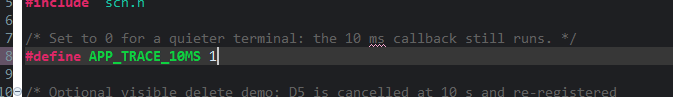
\includegraphics[width=0.9\linewidth]{source/picture/bai_5/lab4_tick_10ms_1.png}
    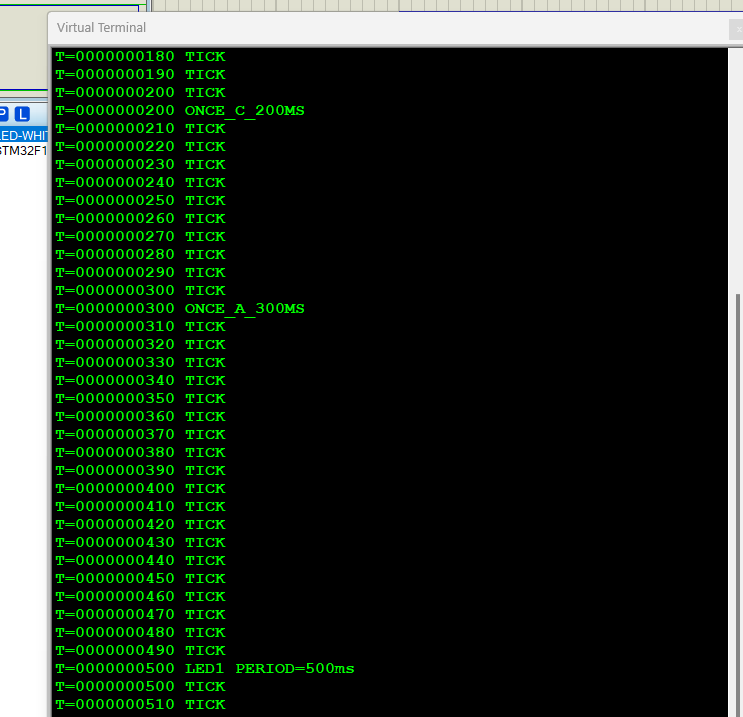
\includegraphics[width=0.9\linewidth]{source/picture/bai_5/lab4_tick_10ms_2.png}
    \caption{10 ms demo: trace macro enabled and consecutive TICK timestamps}
    \label{lab4_tick_10ms}
\end{figure}

Demonstration video: \href{https://github.com/quangnguyencomeng/CO3009-261-CC-2453052/blob/main/Lab/lab_reports/source/vids/lab4_tick_10ms.mp4}{10 ms callback demonstration video}.

\subsubsection{Five periodic tasks with different concurrent intervals}
The first five registrations in \texttt{App\_Init()} have delay and period values of 50, 100, 150, 200, and 250 ticks. Thus, their first executions occur at 500, 1000, 1500, 2000, and 2500~ms and repeat at their respective intervals. LED1 and LED2 share the 1000~ms deadline. At 2000~ms, LED1, LED2, and LED4 are due. The dispatcher calls them sequentially in ID order. Their timestamps can be equal when the callbacks log within the same tick.

The periodic-task video below records the concurrent LED callbacks and their timestamps.

Demonstration video: \href{https://github.com/quangnguyencomeng/CO3009-261-CC-2453052/blob/main/Lab/lab_reports/source/vids/lab4_periodic_tasks.mp4}{Periodic-task demonstration video}.

\subsubsection{One-shot callbacks registered before the main loop}
The application registers A with delay 30, B with delay 10, and C with delay 20 ticks, each with period zero. The timer starts after registration, so the positive delays allow the main loop to begin before these callbacks become due.

\begin{lstlisting}[caption={One-shot callbacks that print their execution timestamps},language=C]
static void shot_a(void) { log_event("ONCE_A_300MS"); }
static void shot_b(void) { log_event("ONCE_B_100MS"); }
static void shot_c(void) { log_event("ONCE_C_200MS"); }
\end{lstlisting}

The expected execution order is B at 100~ms, C at 200~ms, then A at 300~ms. These messages demonstrate ordering by deadline despite the A, B, C registration order. The startup EXPECT message describes the planned sequence; the ONCE messages provide execution evidence.

\begin{figure}[!htp]
    \centering
    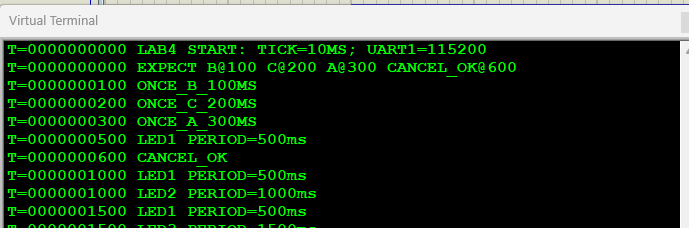
\includegraphics[width=0.9\linewidth]{source/picture/bai_5/lab4_oneshot_cancel.png}
    \caption{One-shot order B, C, A and successful cancellation at 600 ms}
    \label{lab4_oneshot_cancel}
\end{figure}

Demonstration video: \href{https://github.com/quangnguyencomeng/CO3009-261-CC-2453052/blob/main/Lab/lab_reports/source/vids/lab4_oneshot_cancel.mp4}{One-shot and cancellation demonstration video}.

\subsubsection{Testing task deletion}
The application saves the ID of \texttt{should\_not\_run}, which is scheduled at tick 70, and registers \texttt{cancel\_task} at tick 60. Successful deletion produces CANCEL\_OK at 600~ms. The trace should continue past 700~ms with the cancelled callback absent.

\begin{lstlisting}[caption={Deleting a one-shot registration before its deadline},language=C]
static void should_not_run(void) { log_event("FAIL_CANCELLED_TASK_RAN"); }

static void cancel_task(void)
{
    log_event(SCH_Delete_Task(cancelled_id) == SCH_OK ? "CANCEL_OK" : "CANCEL_FAIL");
}
\end{lstlisting}

Figure~\ref{lab4_oneshot_cancel} shows CANCEL\_OK at 600~ms and later output beyond the cancelled 700~ms deadline. The optional visible LED5 scenario is enabled by setting \texttt{APP\_VISIBLE\_DELETE\_DEMO} to one in \texttt{tasks.h}, rebuilding, and loading the new ELF. This stores the LED5 ID and enables stop and restart callbacks at ticks 1000 and 1200.

\begin{lstlisting}[caption={Optional LED5 deletion and re-registration},language=C]
static void stop_led5(void)
{
    if (SCH_Delete_Task(led5_id) == SCH_OK) {
        HAL_GPIO_WritePin(led4_GPIO_Port, led4_Pin, GPIO_PIN_SET);
        log_event("LED5_STOPPED");
    } else log_event("LED5_DELETE_FAIL");
}

static void restart_led5(void)
{
    led5_id = add_checked(task5, 250U, 250U);
    log_event("LED5_RESTART_SCHEDULED");
}
\end{lstlisting}

At 10~s, LED5 toggles before the stop callback because it has the earlier ID for that shared deadline. The stop callback deletes its future registration and forces the LED off. At 12~s, a new LED5 registration is created with a 250-tick initial delay. Its first resumed toggle is at 14.5~s, followed by 17~s. The old 12.5~s release has been cancelled.

\begin{figure}[!htp]
    \centering
    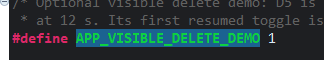
\includegraphics[width=0.9\linewidth]{source/picture/bai_5/lab4_led5_restart_1.png}
    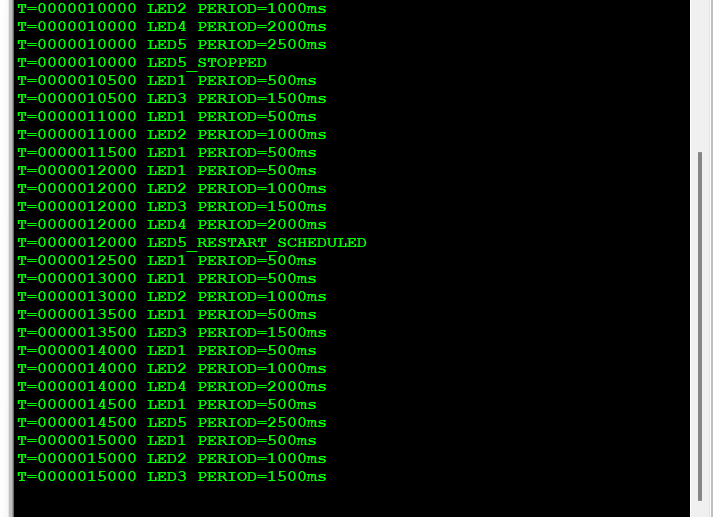
\includegraphics[width=0.9\linewidth]{source/picture/bai_5/lab4_led5_restart_2.png}
    \caption{LED5 demo enabled: stop at 10 s, re-register at 12 s, resume at 14.5 s}
    \label{lab4_led5_restart}
\end{figure}

Demonstration video: \href{https://github.com/quangnguyencomeng/CO3009-261-CC-2453052/blob/main/Lab/lab_reports/source/vids/lab4_led5_restart.mp4}{LED5 deletion and restart video}.

\subsubsection{Discussion of the implementation}
The ordered queue supports multiple pending timeouts, deterministic ordering for equal deadlines, periodic callbacks, and cancellation by ID. Insertion and removal take $O(n)$ time in the main context, while \texttt{SCH\_Update()} takes $O(1)$ in the timer interrupt. Overdue releases are caught up in deadline order, although a long-running callback delays other tasks.

The supplied source has \texttt{APP\_TRACE\_10MS = 0} and \texttt{APP\_VISIBLE\_DELETE\_DEMO = 1}. The 10 ms capture uses \texttt{APP\_TRACE\_10MS = 1}, as shown in its code image. The LED5 capture shows the deletion switch enabled and the expected resumed callback at 14.5~s. Rebuild the matching configuration when reproducing each demonstration.

The handout requests a regular 10~ms tick and also lists interrupt frequencies greater than 10~Hz among unsatisfactory designs. A 10~ms tick corresponds to 100~Hz. This implementation follows the explicit 10~ms tick and callback requirements; the conflicting wording requires instructor clarification if it affects assessment.

\subsection{Submission}

You need to 
\begin{itemize}
    \item Demonstrate your work in the lab class and then
    \item Submit your source code to the BKeL.    
\end{itemize}

\subsection{References}
